\documentclass[10pt,twocolumn]{article}
\usepackage{geometry}
\geometry{verbose,headsep=3cm,tmargin=2.5cm,bmargin=2.5cm,lmargin=2.0cm,rmargin=2.0cm}
\usepackage{graphicx}
\usepackage{xcolor}
\usepackage[font=small]{caption}
\usepackage{amsmath,amssymb,latexsym}
\usepackage{marvosym}
\usepackage{url}
\usepackage{lipsum}
\usepackage{bm}
\usepackage{float}
\usepackage[english]{babel}
\usepackage{hyperref}
\usepackage{subcaption}
\usepackage{subfloat}
\usepackage{epsf}
\usepackage{float}
\usepackage{mathpazo}
\usepackage{pifont}
\usepackage{wrapfig}
\usepackage{multicol}
\usepackage{enumitem}
\usepackage{xcolor}
\usepackage{framed}
\usepackage[utf8]{inputenc}
\graphicspath{{plots/}}
\usepackage{framed}
\usepackage{textcomp}
\usepackage{braket}
\newcommand{\highlight}[1]{%
  \colorbox{orange!50}{$\displaystyle#1$}}
% Default fixed font does not support bold face
\DeclareFixedFont{\ttb}{T1}{txtt}{bx}{n}{10} % for bold
\DeclareFixedFont{\ttm}{T1}{txtt}{m}{n}{10}  % for normal

% Custom colors
\usepackage{color}
\definecolor{deepblue}{rgb}{0,0,0.5}
\definecolor{deepred}{rgb}{0.6,0,0}
\definecolor{deepgreen}{rgb}{0,0.5,0}

\usepackage{listings}

% Python style for highlighting
\newcommand\pythonstyle{\lstset{
language=Python,
basicstyle=\ttm,
otherkeywords={self},             % Add keywords here
keywordstyle=\ttb\color{deepblue},
emph={MyClass,__init__},          % Custom highlighting
emphstyle=\ttb\color{deepred},    % Custom highlighting style
stringstyle=\color{deepgreen},
frame=tb,                         % Any extra options here
showstringspaces=false            % 
}}


% Python environment
\lstnewenvironment{python}[1][]
{
\pythonstyle
\lstset{#1}
}
{}

% Python for external files
\newcommand\pythonexternal[2][]{{
\pythonstyle
\lstinputlisting[#1]{#2}}}

% Python for inline
\newcommand\pythoninline[1]{{\pythonstyle\lstinline!#1!}}
% Document font:
\usepackage{charter}

\begin{document}

%%% HEADER --------------------------------------------------------------
% ------------------------------------------------------------------------

\twocolumn[{
\begin{@twocolumnfalse}

  \begin{center}
%\textcolor{lgray}
    \vskip-5em

    \hfill
    \fontsize{10}{10}\selectfont {\textit{Bruxelles, June 2020}}
    \vskip2ex
	\vspace{5ex}
    \fontsize{20}{10}\selectfont {The tensor necessity}
      \vspace{1ex}
      
      \fontsize{16}{10}\selectfont {- a short story about momentum transport in fluids}
  \noindent%
    
\vskip1ex

{\rule{\textwidth}{0.5pt}}

  \end{center}
  
    \fontsize{7}{10}\selectfont {This work is licensed under the Creative Commons Attribution-NonCommercial-ShareAlike 4.0 International (CC BY-NC-SA 4.0) license.}

\vspace{6mm}

\end{@twocolumnfalse}
}]

%%% HEADER END -----------------------------------------------------------
% ------------------------------------------------------------------------

\vspace{10mm}

\setlength{\parindent}{0cm}

\fontsize{14}{10}\selectfont {Kamila Zdybał}

\vspace{2mm}

\fontsize{8}{10}\selectfont {\textit{Université libre de Bruxelles, kamila.zdybal@ulb.ac.be}}

\fontsize{8}{10}\selectfont {\textit{camillejr.github.io/science-docs, kamila.zdybal@gmail.com}}

\section*{Preface}

At first encounter, tensors can seem like strange mathematical objects. It can be challenging to grasp their meaning and their relevance might not be immediately obvious. At the same time, tensors are indispensable when studying fluid dynamics. So what's with the tensors and why do we need them?

\,\,

In this document I would like to convince you that we necessarily need tensors in fluid dynamics! Using a simple example of a Couette flow we will motivate their usefulness. Hopefully by the end of this document you will find tensors very useful mathematical objects that make our life easier. Join me on the journey!

\,\,

Please feel free to contact me with any suggestions, corrections or comments.

\section*{Keywords}

\textit{tensor, momentum transport, transport phenomena, fluid dynamics, Couette flow}

%\tableofcontents


\section*{Viscous momentum flux tensor}

We will begin our journey with an illustrative example to build our intuition around tensor quantities. We will take a quite simple example of a Couette flow - flow between two parallel plates, one being stationary and one moving with a velocity $\mathbf{u}$ as presented in Figure \ref{fig:couette-flow}.
\begin{figure}[H]
\centering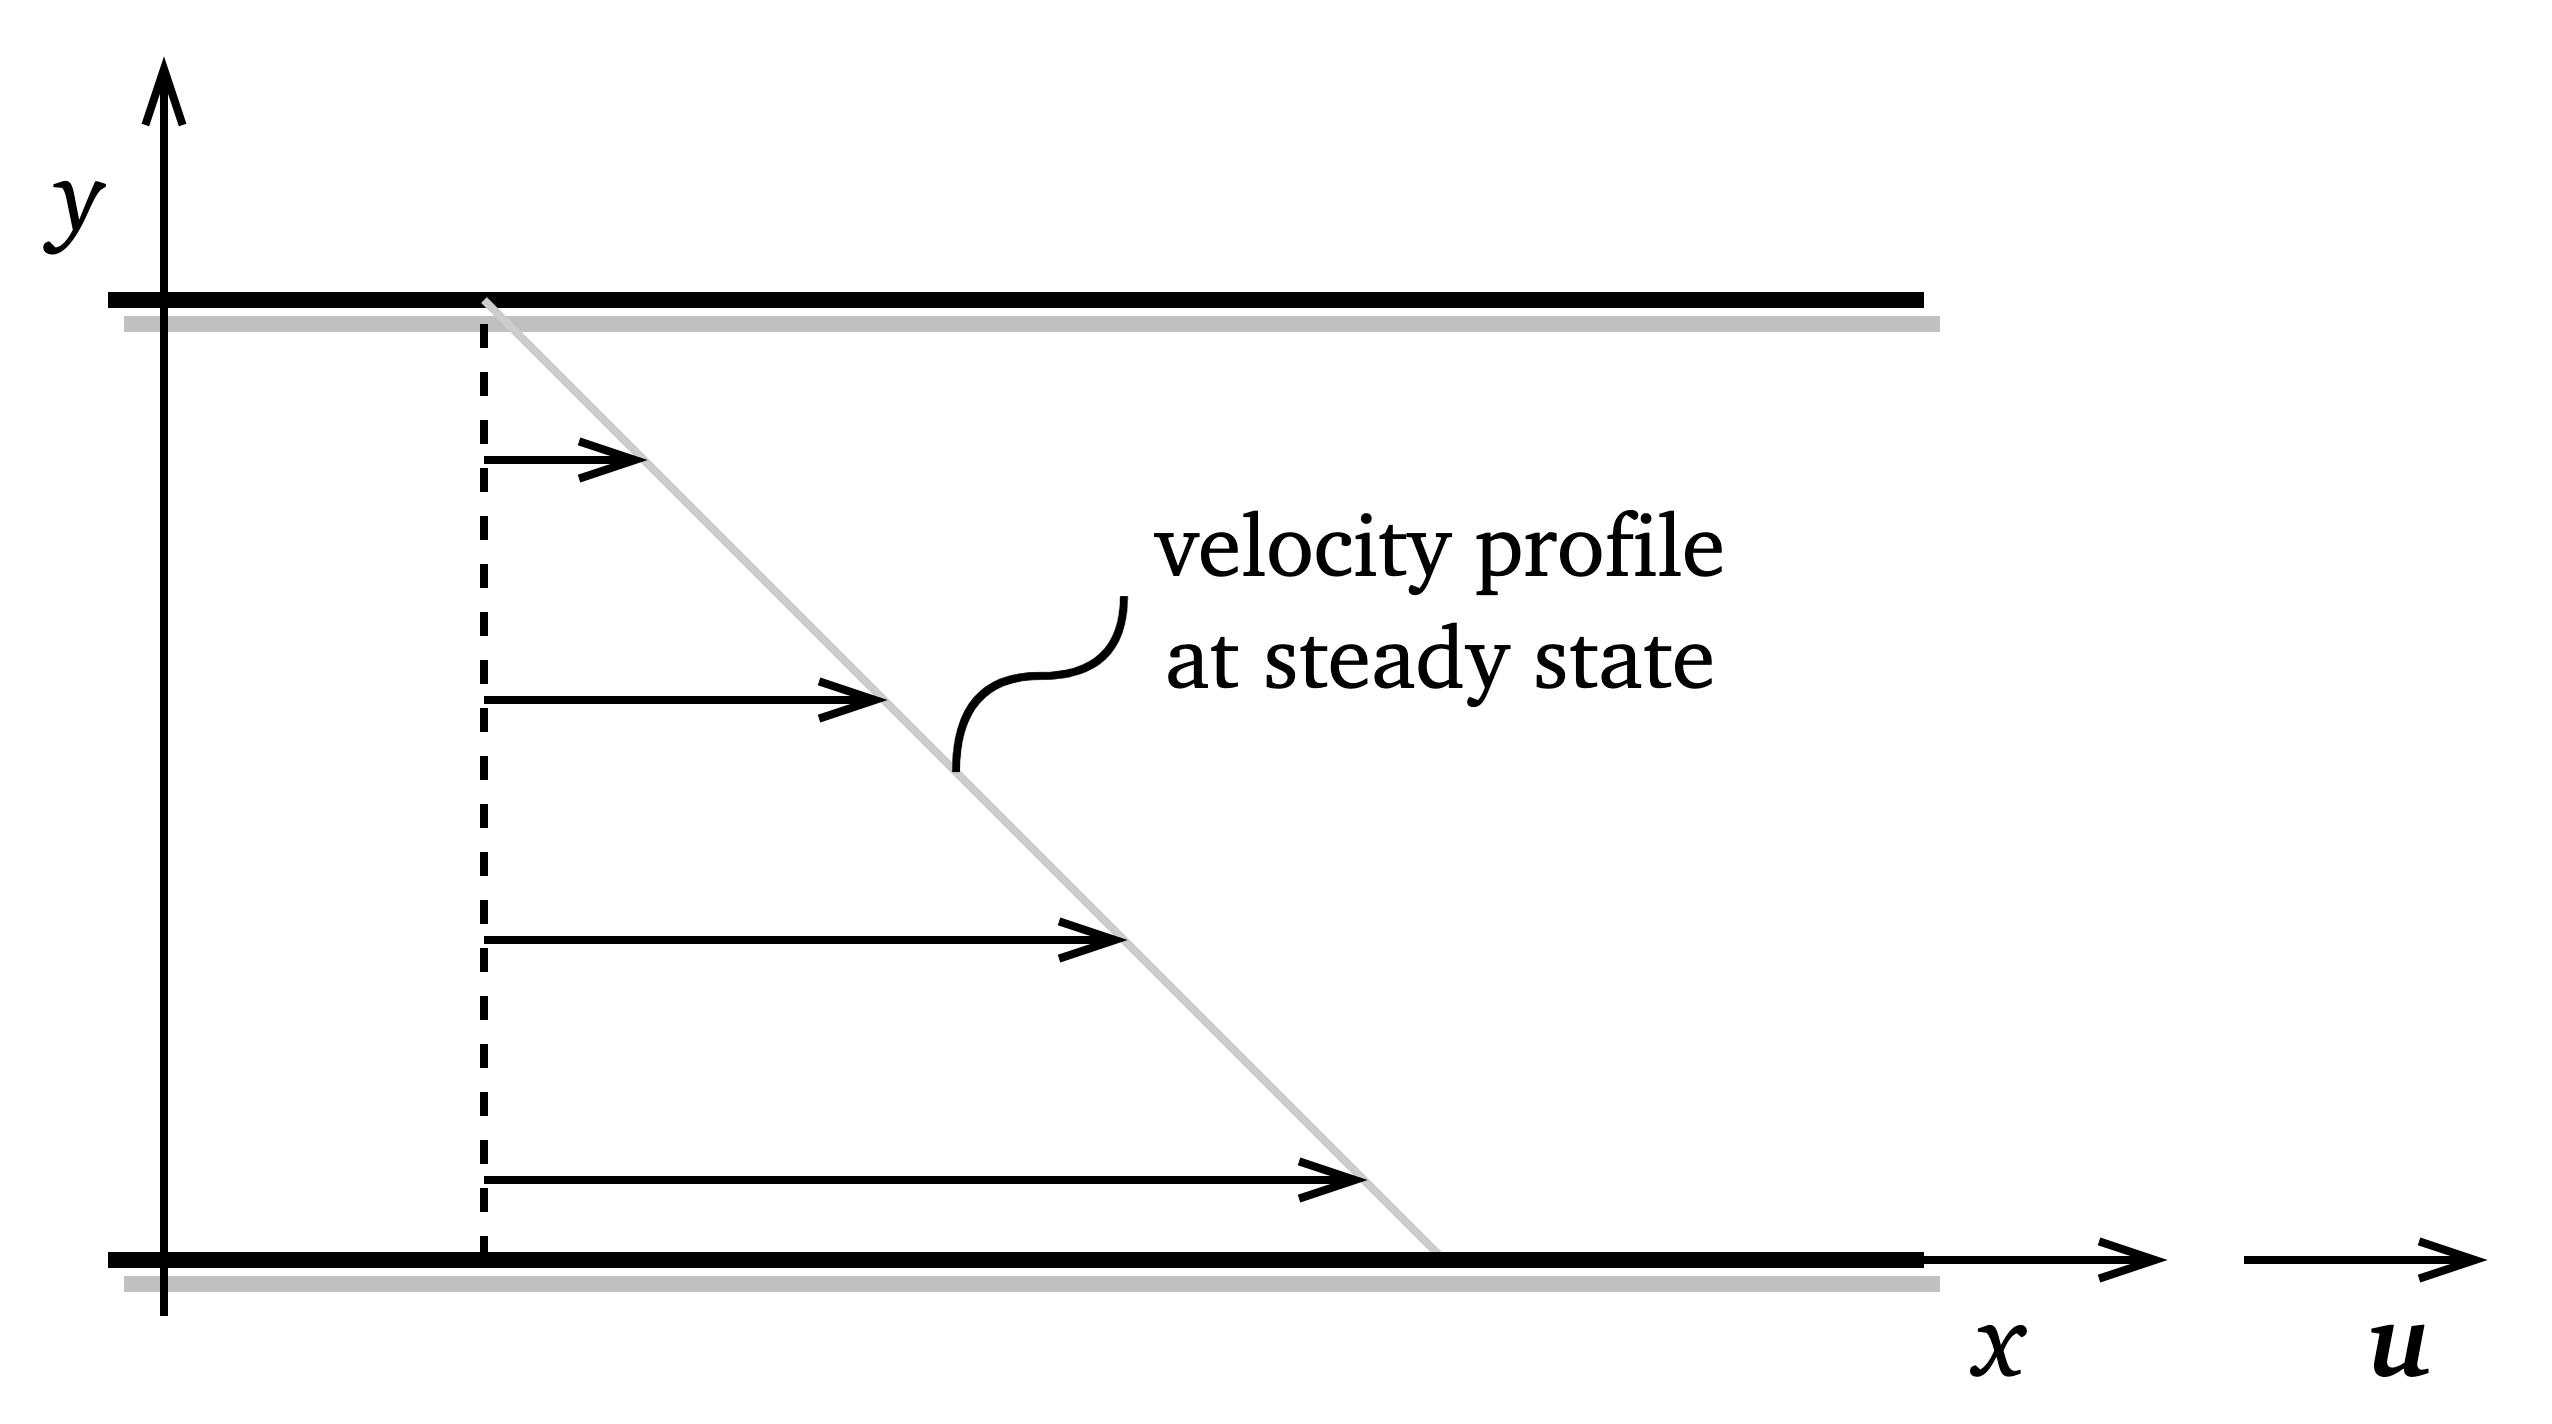
\includegraphics[width=7cm]{couette-flow.png}
\caption{Velocity profile in the Couette flow.}
\label{fig:couette-flow}
\end{figure}
Suppose that we first start with the initial situation when both plates are stationary and at some moment in time we begin moving the bottom plate reaching velocity $\mathbf{u}$ after a while. You may already expect that the moment we started moving the plate something interesting starts to happen in the fluid in-between - it begins moving as well. As the flow develops, the moving plate successively "drags" fluid particles in a layer adjacent to the plate. Once those fluid particles are set in motion in the positive $x$-direction, the moving layer of fluid "drags" another layer laying directly on top of it. This "dragging" progresses upwards, in the positive $y$-direction, until at the top stationary plate the fluid is stagnant again. After a sufficient amount of time the situation becomes steady - the velocity profile is fully developed and does not depend on time. The steady state velocity profile is plotted in Figure \ref{fig:couette-flow} as well - it is a linear function of $y$ which is something that we will not prove here.

\begin{wrapfigure}{R}{0.1\textwidth}
\centering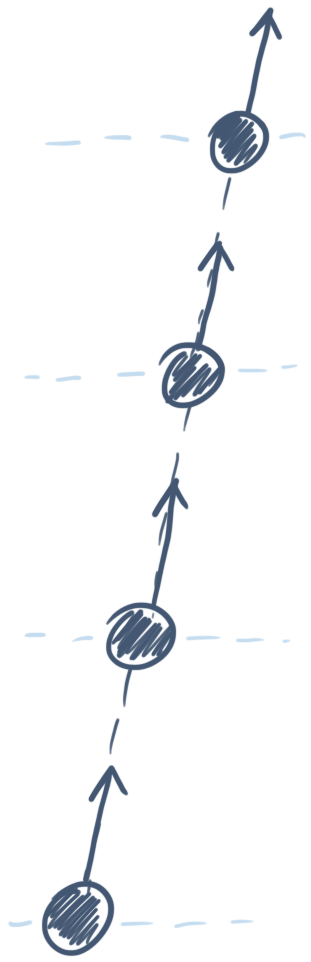
\includegraphics[width=1.8cm]{molecular-collisions.png}
\label{fig:molecular-collisions}
\end{wrapfigure}
If we assume that the fluid flow between plates is laminar we may, perhaps a bit naively, assume that fluid flows in thin "laminates" stacked one on top of the other. Knowing the velocity profile, we know exactly what the velocity of each laminate is (at any position $y$). In general, laminate at a lower $y$ coordinate will have a larger velocity than laminate at a larger $y$ coordinate\footnote{That holds in our case where we assumed that it's the bottom plate that is moving and velocity decreases to zero once we reach the top plate. Similar reasoning can be done assuming that the top plate is moving at velocity $\mathbf{u}$ and the bottom one is stationary.}.
In Figure \ref{fig:momentum-transport-in-laminates} we have drawn three such laminates, each having thickness $dy$.
Knowing the velocities, we also know the momentum carried by each laminate. We will in fact consider specific momentum for the purpose of this discussion which is momentum per unit volume. Let's look at the situation from the perspective of one of the laminates whose $y$-coordinate is simply denoted $y$. Its specific momentum is $\rho \mathbf{u}|_{y}$.  It gains momentum from the faster moving laminate directly below whose specific momentum is $\rho \mathbf{u}|_{y-dy}$. It also looses momentum to the slower laminate directly above it whose specific momentum is $\rho \mathbf{u}|_{y+dy}$. Such "transport" of momentum is in practice possible due to molecular collisions. Since every collision is an opportunity to exchange momentum, when molecules from one laminate collide with molecules from another laminate, momentum can be transported in the positive $y$-direction. 

\begin{figure}[H]
\centering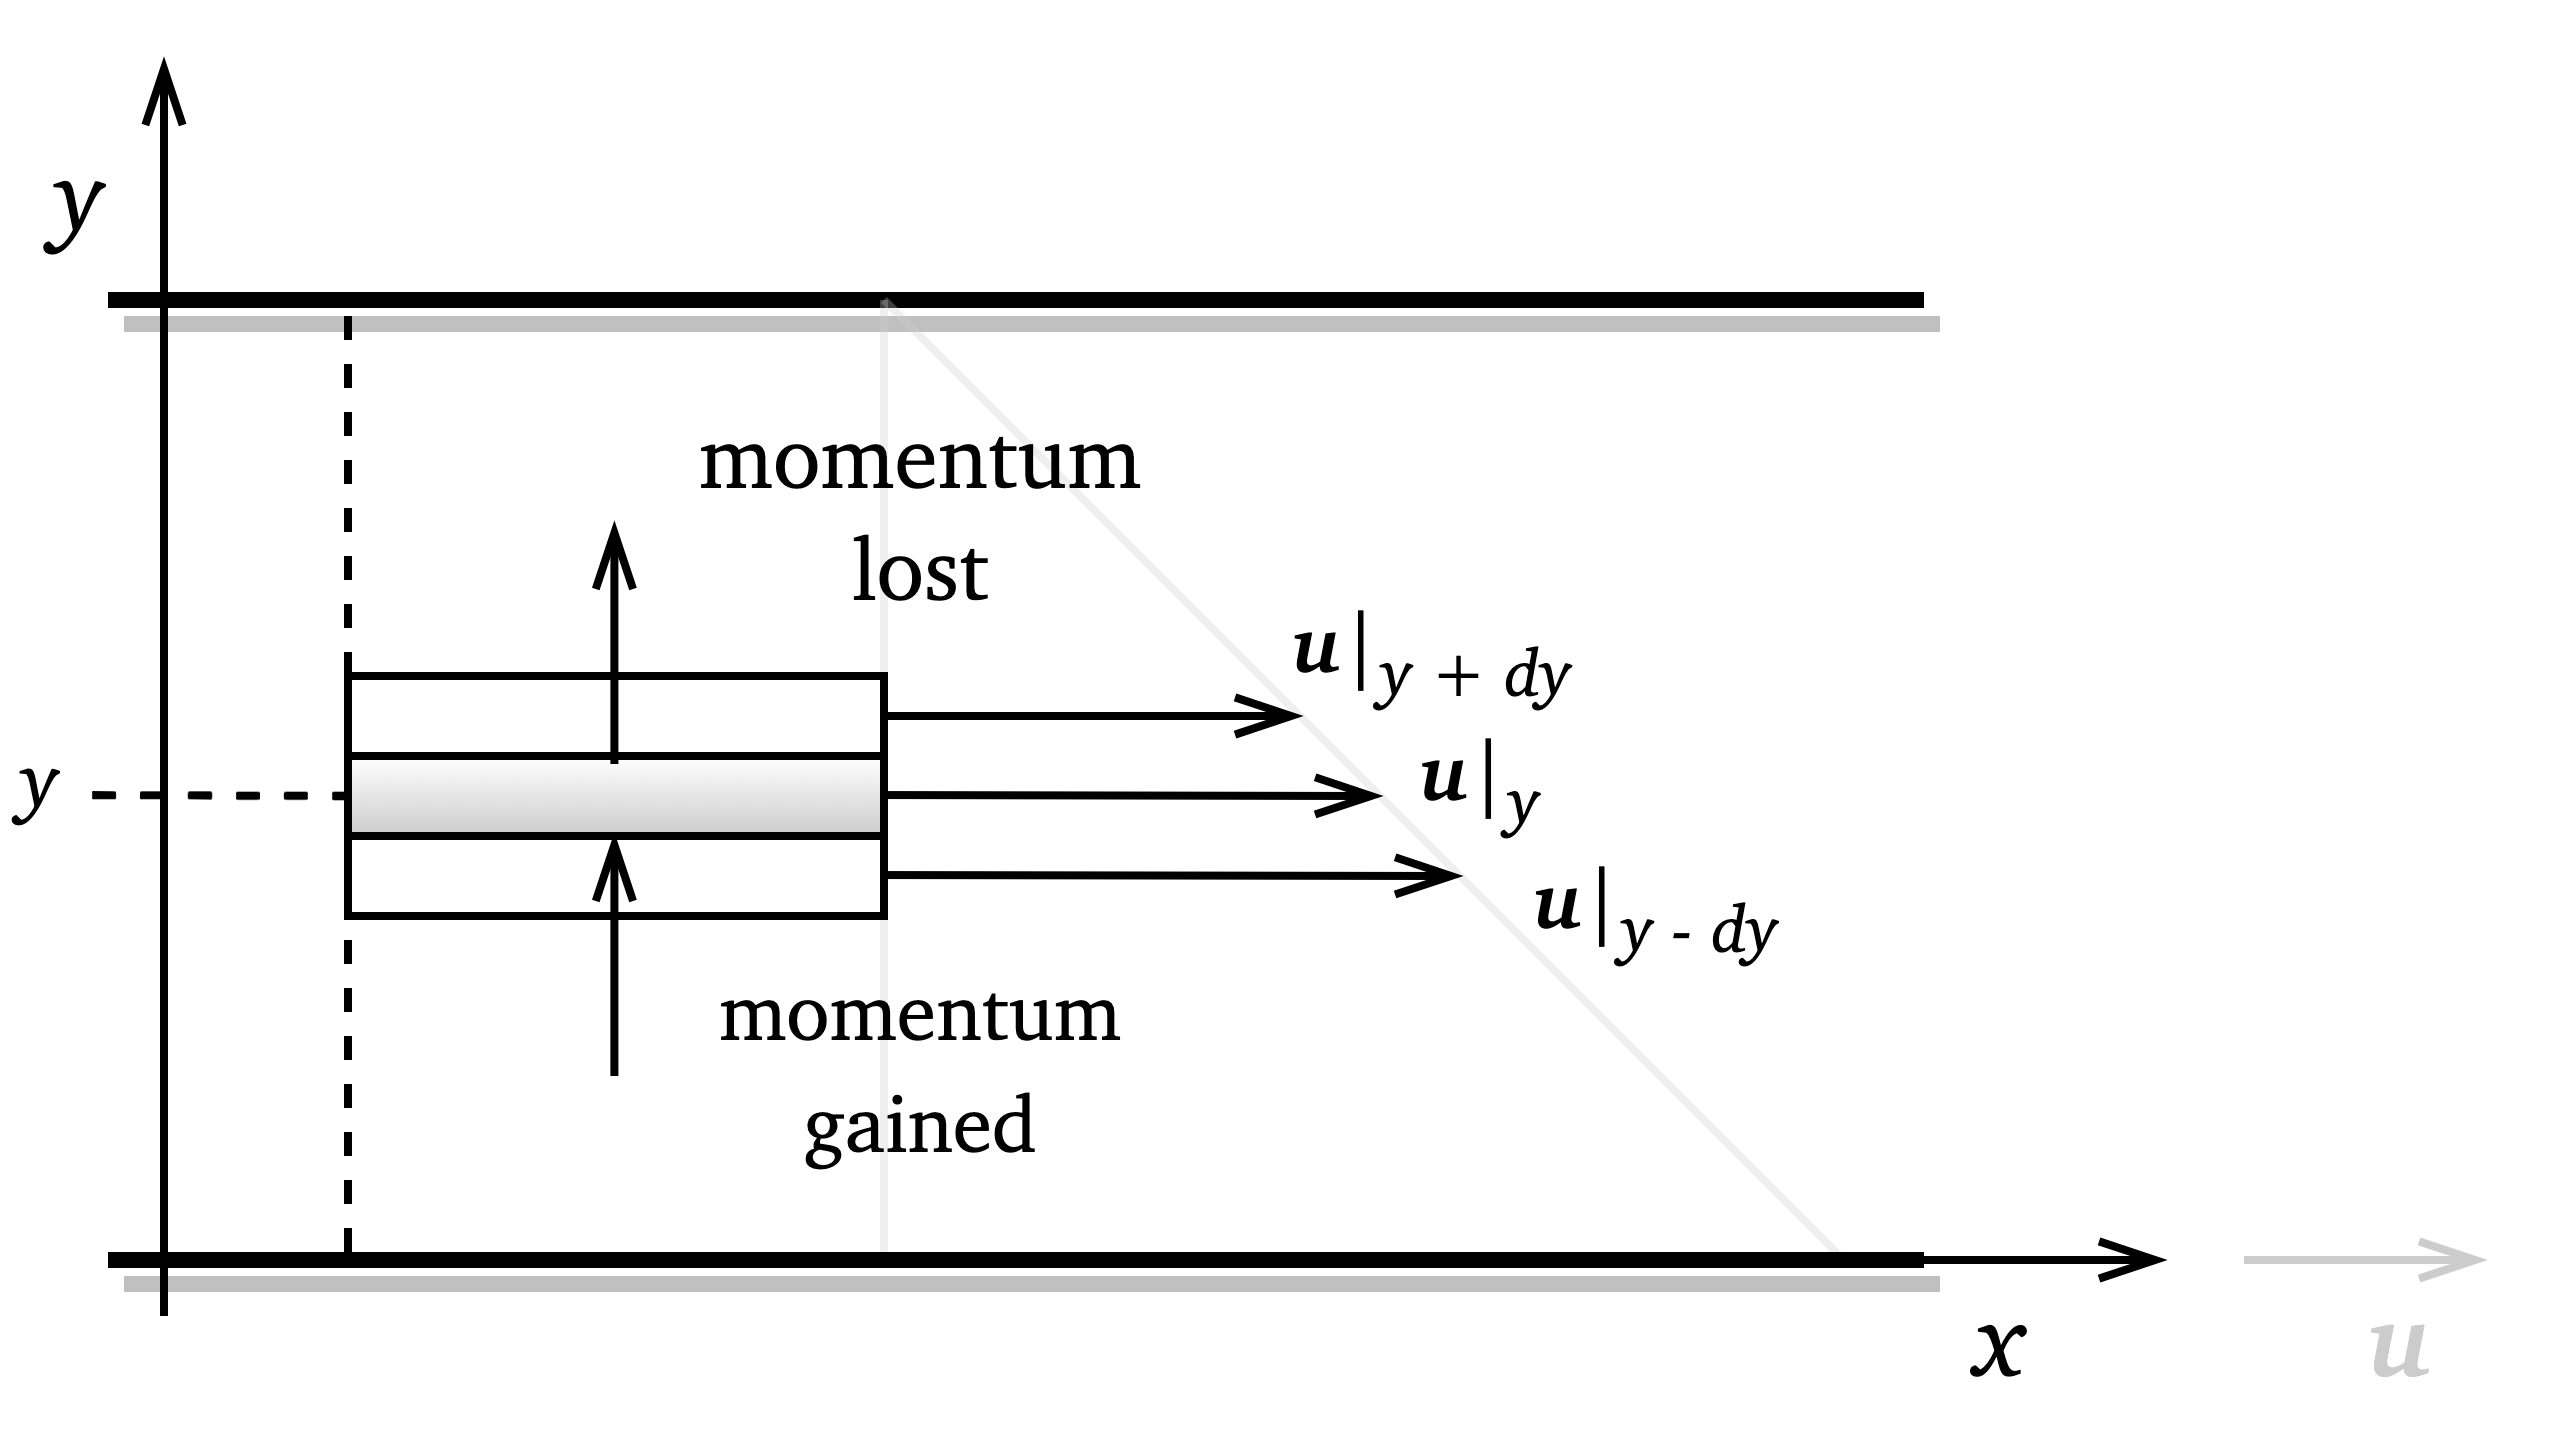
\includegraphics[width=7cm]{momentum-transport-in-laminates.png}
\caption{Transporting momentum between fluid "laminates".}
\label{fig:momentum-transport-in-laminates}
\end{figure}
The "dragging" that we talked about before is thus achieved by momentum transport - a faster moving laminate gives some of its momentum to the slower moving one. Note that this can only happen in the world with friction! Since in fluids friction is accounted for by viscosity it becomes clear that viscosity plays a role in transporting momentum\footnote{Although in a "frictionless world" momentum can still be transported by a fluid but not by means of viscosity. We will move to other forms of momentum transport in the next section.}.
\begin{figure}[H]
\centering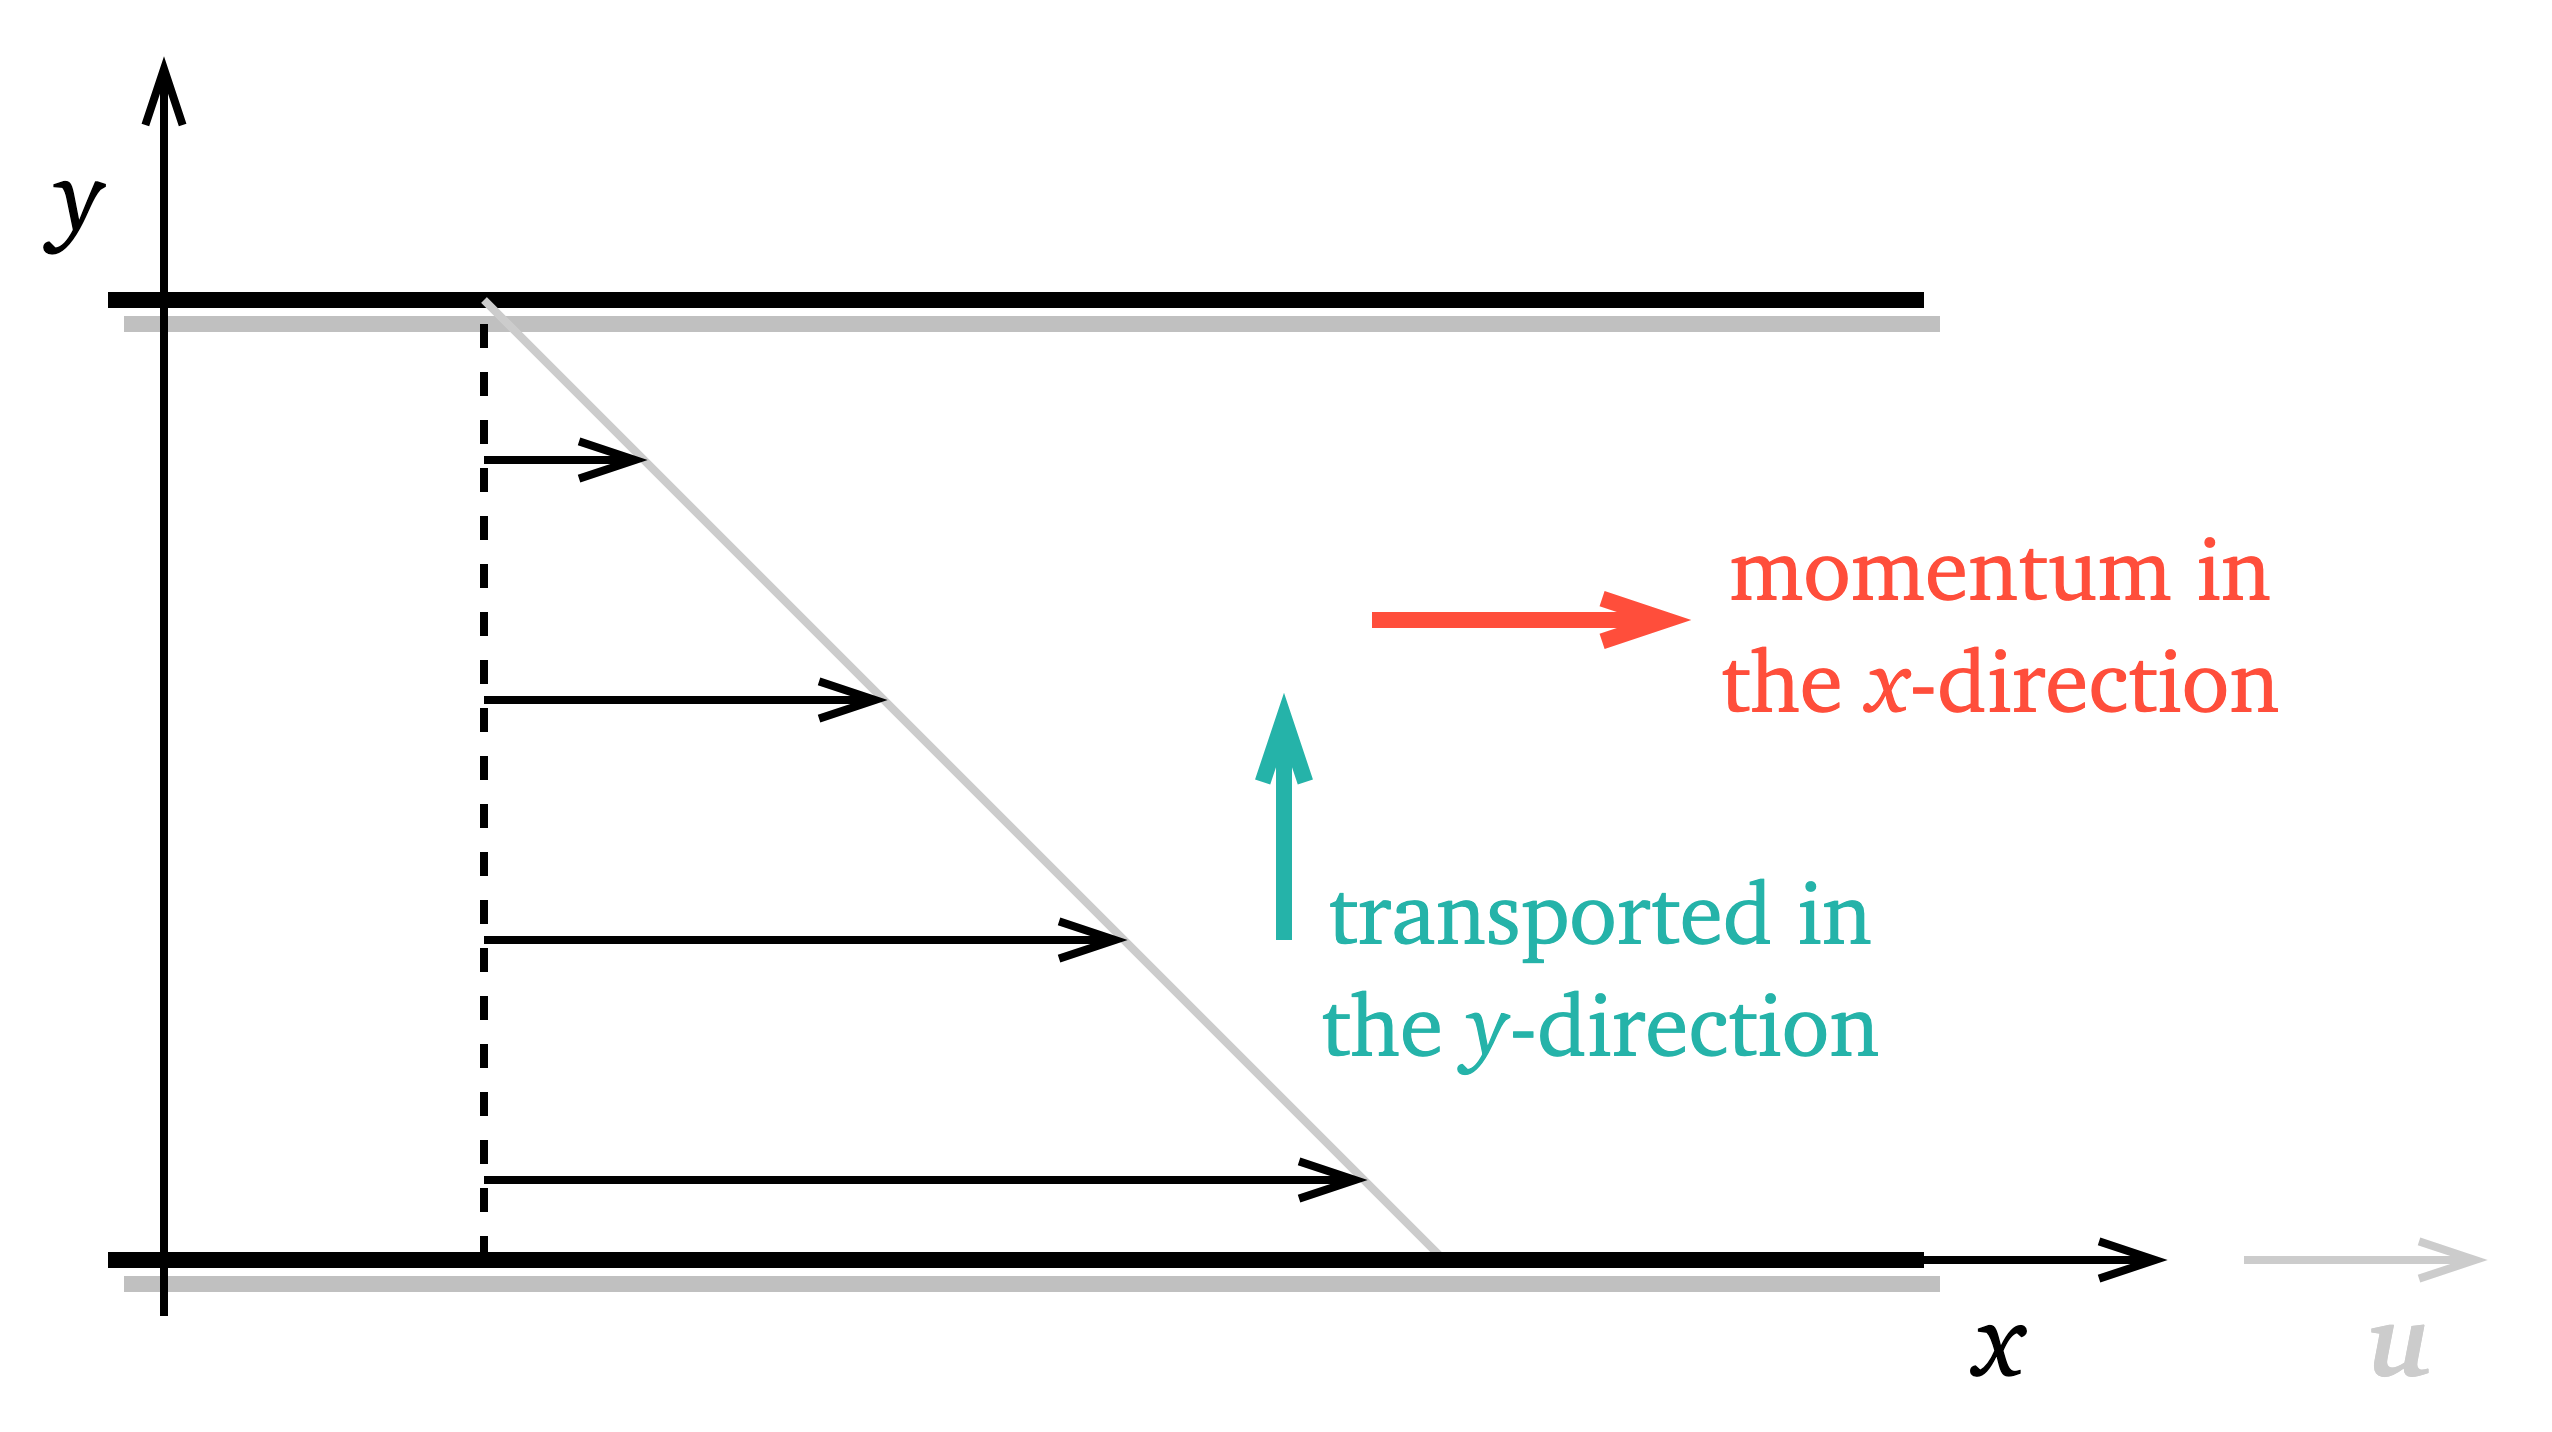
\includegraphics[width=7cm]{couette-flow-momentum-transport.png}
\caption{Momentum transport in a Couette flow.}
\label{fig:couette-flow-momentum-transport}
\end{figure}
An important concept now emerges. Momentum is a vector quantity that has a direction of the velocity vector. In our simple example of the Couette flow, momentum of every laminate has direction parallel to the $x$-axis (in accordance with the velocity profile). However, as we have reasoned before, the transport of that momentum is happening in the direction parallel to the $y$-axis. This is conceptually presented in Figure \ref{fig:couette-flow-momentum-transport}. 

\begin{wrapfigure}{L}{0.2\textwidth}
\centering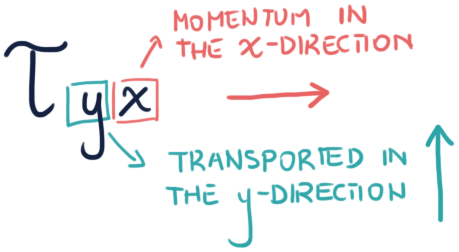
\includegraphics[width=3cm]{tau_y_x.png}
\label{fig:tau_y_x}
\end{wrapfigure}
Such transported momentum (also called \textit{momentum flux}) is denoted with a symbol $\tau_{yx}$. Notice now that this quantity is carrying information about two directions - one telling us which direction is the momentum vector pointing and the other telling us which direction that momentum is being transported. If we considered a different system, perhaps there would be momentum in the $x$-direction transported in the $z$-direction, or maybe momentum in the $y$-direction transported in the $x$-direction\footnote{Can you think of situations when momentum in the $x$-direction is transported in the $x$-direction?}.

Tensors are objects that keep track of exactly that - they allow to associate more than one direction to a physical quantity. In the case of a Couette flow considered here, the tensor quantity $\tau$ would be called \textit{second-order tensor} because it carries information about two directions. This can be thought of as a further extension to the concept of a vector, which is characterized by a magnitude and a direction. Tensor is characterized by a magnitude and possibly multiple directions attached to it. Of course, we need to create such notation that we know what each direction means physically. Hopefully now you can appreciate that tensor is a very useful tool in fluid dynamics, where vector quantities can be transported in many directions!

For instance, in a three-dimensional world, momentum vector can be in general pointing in any of the three directions $x$, $y$ or $z$, and transported in any of the three directions $x$, $y$ or $z$. Tensors allow us to keep track of all those directions as well. If we wanted to account for all these possibilities we would need $3 \times 3 = 9$ quantities $\tau_{ij}$. For convenience, we often write out the elements of a tensor in a form of a table that resembles a matrix. Unlike in a scalar matrix, this table has additional information attached to every element - the directions represented. Figure \ref{fig:tensor-in-matrix-form} shows an example of the most general second-order tensor that could represent viscous momentum flux in a three-dimensional fluid flow. We note the directions that each element is keeping track of. Once we write down a specific $\tau_{ij}$, its directions can be understood through the indices $i$ and $j$. In the case of a Couette flow we needed only one of those elements - $\tau_{yx}$ - since there was only one direction for momentum and only one direction in which that momentum was transported.

\begin{figure}[H]
\centering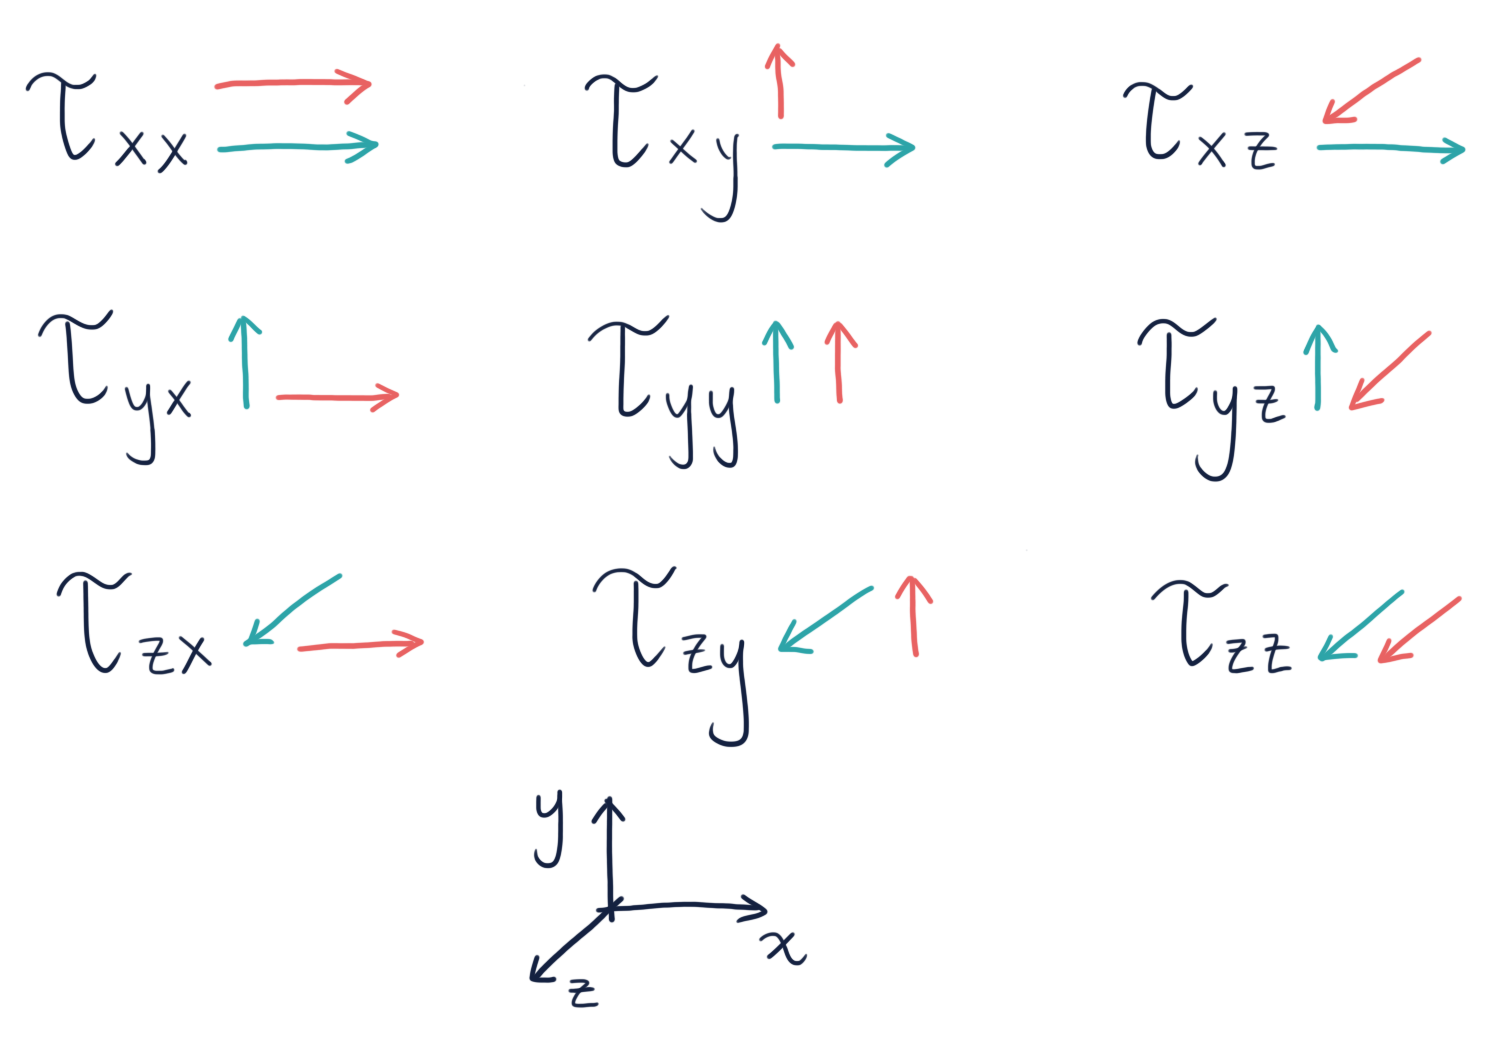
\includegraphics[width=8cm]{tensor-in-matrix-form.png}
\caption{Second-order tensor from a three-dimensional world.}
\label{fig:tensor-in-matrix-form}
\end{figure}


%\section*{Convective momentum flux tensor}

%Transport of a vector quantity is not the only application for a tensor. Another possibility could be keeping track of a vector quantity that is linked to a surface oriented in a particular direction (with the direction being defined by a unit normal vector). Imagine then having unit normal vectors in Cartesian coordinates $\hat{i}$, $\hat{j}$ and $\hat{k}$ that specify surfaces perpendicular to respectively $x$, $y$ and $z$ axis. At each of those surfaces 








%\section*{Operations on tensors}



\vspace{5mm}

%\section*{Epilogue}

%Some say that a good scientific writing that keeps the reader engaged is characterized by a single idea carried over from sentence to sentence that guides the reader through the journey. I hope that I managed to make this reading interesting to you by transporting the idea of a tensor downward this document!

%I wanted to use the momentum transport as a pretext to explain these bizzare objects that tensors are and I hope that I managed to make tensors the main character of this article. On the other hand, momentum transport in fluids has itself its peculiarities. Hopefully piggybacking the concept of a tensor was an overall useful experience for you!
















\thebibliography{}

\bibitem{BSL} R.B. Bird, W.E.Stewart, E.N. Lightfoot, \textit{Transport Phenomena}, John Wiley \& Sons, Inc., 2001

\end{document}